\section{Firewalls, Intrusion Detection \& Evasion}

\subsection{Firewalls}

A firewall is a system used to protect or separate a trusted network from an untrusted network, while allowing authorized communications to pass from one side to the other.

\begin{itemize}
	\item \textbf{Network Firewall:} Network firewalls are a software appliance running on specific hardware or as virtual instance that filter traffic between two or more networks. Protect different network segments.
	\item \textbf{Host Firewall:} Host-based firewalls provide a layer of software on one host that controls network traffic in and out of	that single machine. Protect single machine
\end{itemize}

\paragraph{Hostbased vs Network:} Host based firewalls have context, know exactly what is running on a host. This allows for more fine-grained decisions. Host based firewalls are good for mobile devices (e.g. phones). Network firewalls are good if you e.g. can't install a firewall on a device (e.g. printer).

\paragraph{Filtering Rule:} Firewall rules are processed in order: the first rule that matches is picked. Thus, ordering of rules is very important.
\begin{itemize}
    \item Ingress: Filter incoming traffic (from low security to high security)
    \item Egress: Filter outgoing traffic (often gets forgotten)
    \item Default Policy: Define what to do when no rule matches (default accept vs. default reject)
    \item Deny Access: Tehniques to deny access: DROP silently drop packet (port scanner think its open), REJECT drop packet and inform sender (ICMP message).
\end{itemize}

\paragraph{Firewall State:}
\begin{itemize}
	\item \textbf{Stateless Firewall:} look at each packet on the network layer individually, no state maintained. Decisions based on packet header information. This is fast, scalable and simple but very limited.
	\item \textbf{Stateful Firewall:} keep also track of the state of the network connections, decision also based on session state. This is more powerful but: state explosion, inconsistencies, state for UDP? The problem with state explosion: an attacker can exhaust the memory of a firewall. Then, the default rule matches: if default accept: all traffic is allowed. If default deny: server is DoSed.
\end{itemize}

\paragraph{Evolution of Firewalls:} The legacy firewall technology is effectively blinded by the evolution:
\begin{itemize}
    \item Firewalls can't block all malicious traffic, many ports must be kept open for legitimate applications.
    \item Users unwittingly download dangerous applications or other forms of malicious code
    \item Peer-to-peer and instant messaging have introduced new infection vectors.
    \item Web 2.0 trends push critical business applications through firewall ports that were previously reserved for a single function (e.g. HTTP)
\end{itemize}

\paragraph{Next Generation Firewall (NGFW)}

\textbf{Functionality:} deep packet (content) inspection, take application and protocol state into
account for security decision. This allows for even more powerful rules, protocol and application awareness but requires support for many (badly documented) protocols, has performance and scalability issues and introduces inconsistencies between host/app and FW.

\paragraph{Web Application Firewall (WAF)}

Protect web-based applications from malicious requests. Request filtering: request pattern, SQL injection, XSS, buffer overflow attempts, etc. Often implemented as a reverse proxy. Static or dynamic blacklisting/whitelisting. False positive problem. WAF's are often implemented as a reverse proxy to protect public facing web applications. Reverse Proxy: client accesses reverse proxy without knowing internal network. Reverse proxy then manages resources from internal network for client.

\paragraph{Organizational Challenges}

Managing and maintaining firewall rules in a company is challenging. Firewall rules are complex and if the employee that created them leaves, someone else has to understand the monster. Further, security and network operation teams have opposing interests: security team wants to provide secure access, network team wants to provide high availability.

\paragraph{}{Firewall Attack Methods}
\begin{itemize}
    \item IP Source Spoofing: spoofing src addr to bypass filters
    \item Artificial Fragmentation: of packets to bypass rules (firewall needs to reassemble to understand content), also out of sequence sending of fragments.
    \item Denial of Service: Firewall state explosion, whats fallback policy?
    \item Encodings: Different encodings and addition of noise (different obfuscation techniques). Undefined or border cases are very effective for detection evasion.
    \item Vulnerabilities: Firewalls are complex software, which are riddled by vulnerabilities as any other software product.
\end{itemize}

\subsection{Intrusion Detection \& Prevention}

Protecting a large number of hosts, end-points, or network segments is not trivial.
\begin{itemize}
    \item Reactive: system can only detect already known attacks
	\item Proactive: system can detect known and yet unknown attacks
	\item Deterministic: system always performs the same given the same input (blacklist, signatures)
	\item Non Deterministic: system detection is fuzzy (heuristics, machine	learning, sandboxing) and depends on current state of the world. The reason for alert is typically not known.
\end{itemize}

\paragraph{Detection Techniques}

\begin{itemize}
    \item Protocol Analysis: Analysis and decoding of protocols. Reassembly and normalization of traffic
	\item Signature based systems (static): Promptly identify and label threat. But I can only identify threats that I've already seen before. For each new threat, a unique signature or signature artifact is created by a skilled engineer or security researcher. Frequent updates to signature database or online lookups.
	\begin{itemize}
		\item One-Dimensional: blacklist/ whitelist (e.g based on MD5 hashes). This is fast and low rate of false positives. But it's reactive and needs frequent updates.
		\item Two-Dimensional: classic regular-expression functions and string matching. This is more flexible and has low FPR and low/medium resource requirements. More flexibility but it's still reactive and needs frequent updates.
		\item Multi-Dimensional: instead of triggering on a single signature, a	multi-dimensional signature was created. More efficient and effective than single approach. hybrid of two above methods
	\end{itemize}
	\item Sandboxing: Run (potential) malware in a VM and examine its behavior. This is proactive and doesn't need signature updates but is resource intensive and difficult to scale. Malware can further evade sandboxing (e.g. malware could wait for 3 days before becoming malicious).
	\item Machine Learning: Apply supervised and unsupervised machine learning algorithms to detect malicious traffic, malware, etc. Problem with SL models: training data \textit{needs} to be clean (no unknown attacks), otherwise the SL model learns something wrong. With USL models, interpretability is an issue (also with SL).
\end{itemize}

\paragraph{Decision Making}

This faces many challenges: encrypted traffic (can't inspect content, only headers and statistical analysis), high number of false positives, high link speeds, induced latency, application level attacks (JavaScript, ..), etc.
\\
Accurate = right direction, on target. Precise = clustered values with low scatter.\\

\textit{“It is better to be roughly right than precisely wrong.”}\\

\begin{itemize}
	\item \textbf{0\% FNR:} Always predict 'Attack!'
	\item \textbf{0\% FPR:} Always predict 'No attack!
\end{itemize}

The difficulty: Build a detector with optimal balance between FP and FN. FNR and FPR should never be considered in isolation. Ideally, consider a joint detection metric such as the F1 score.\\
Accurate detection is very challenging when rate of attacks is very low. If we have lots of traffic but very few attacks, we'll have lots of false positives, which lowers trust in the detector. 

\paragraph{Detection Evasion}

\paragraph{Malware Development Lifecycle}
\begin{enumerate}
	\item Develop new malware with desired functionality
	\item Automatically create numerous permutated samples of the initial malware at massive scale:
	\item Protect samples from analysis:
	\begin{itemize}
		\item Use \textit{crypter} to encrypt malware s.t. detection systems and static analysis processes are ineffectual.
		\item Upon execution only decrypt sections of code that are in the process of being executed on the victim’s computer.
		\item Use \textit{packers} to make binary files smaller (faster infection), make it more difficult for AV to detect malicious payload. Advanced packers employ polymorphic output capabilities (restructure malware binary everytime it's executed)
	\end{itemize}
	\item Make samples aware of sandboxing/detection technologies
	\begin{itemize}
		\item Use \textit{protector} to add anti-debugging features to malware that prevent security researchers and automated sandbox analysis technologies from dissecting samples.
		\item “protector” technology was originally designed as a DRM protection technology
		\item Protectors detect the use of debuggers or virtualization techniques if seen, the malware then causes different operations
	\end{itemize}
	\item Quality Assurance: Test samples against all current anti-malware solutions before deployment (if sample is detected by antivirus: \texttt{goto 2}):
	\begin{itemize}
		\item Check if the malware is detected by common AV software. Only testing services that do not submit malware samples to antivirus vendor are used (otherwise the malware would already be known).
	\end{itemize}
\end{enumerate}

The malware used in a targeted attack will not be detected by anti-malware tools at the time of attack because it was tested beforehand.

\paragraph{Polymorphism Techniques}
Mutate code while keeping the original algorithm intact. Swapping equivalent code constructs, changing the order of code, insert noise, compiler modulation. Also swapping of registers, reordering of instructions and defining functions in a different order.

\textbf{Binders:} Binders are used by malware authors to “embed” and Trojan other software packages (e.g. add trojan to Adobe Photoshop torrent). This helps to propagate malware, trick users into downloading and executing seemingly legit software. 

\paragraph{Attack Detection \& Defense Effectiveness}

\begin{itemize}
    \item Unable to inspect encrypted traffic
    \item High number of false positives
    \item Latency introduced by inspection engine
    \item Application level attacks (JavaScript,...)
    \item Policy/signature management
\end{itemize}

\begin{minipage}{\linewidth}
    \centering      
    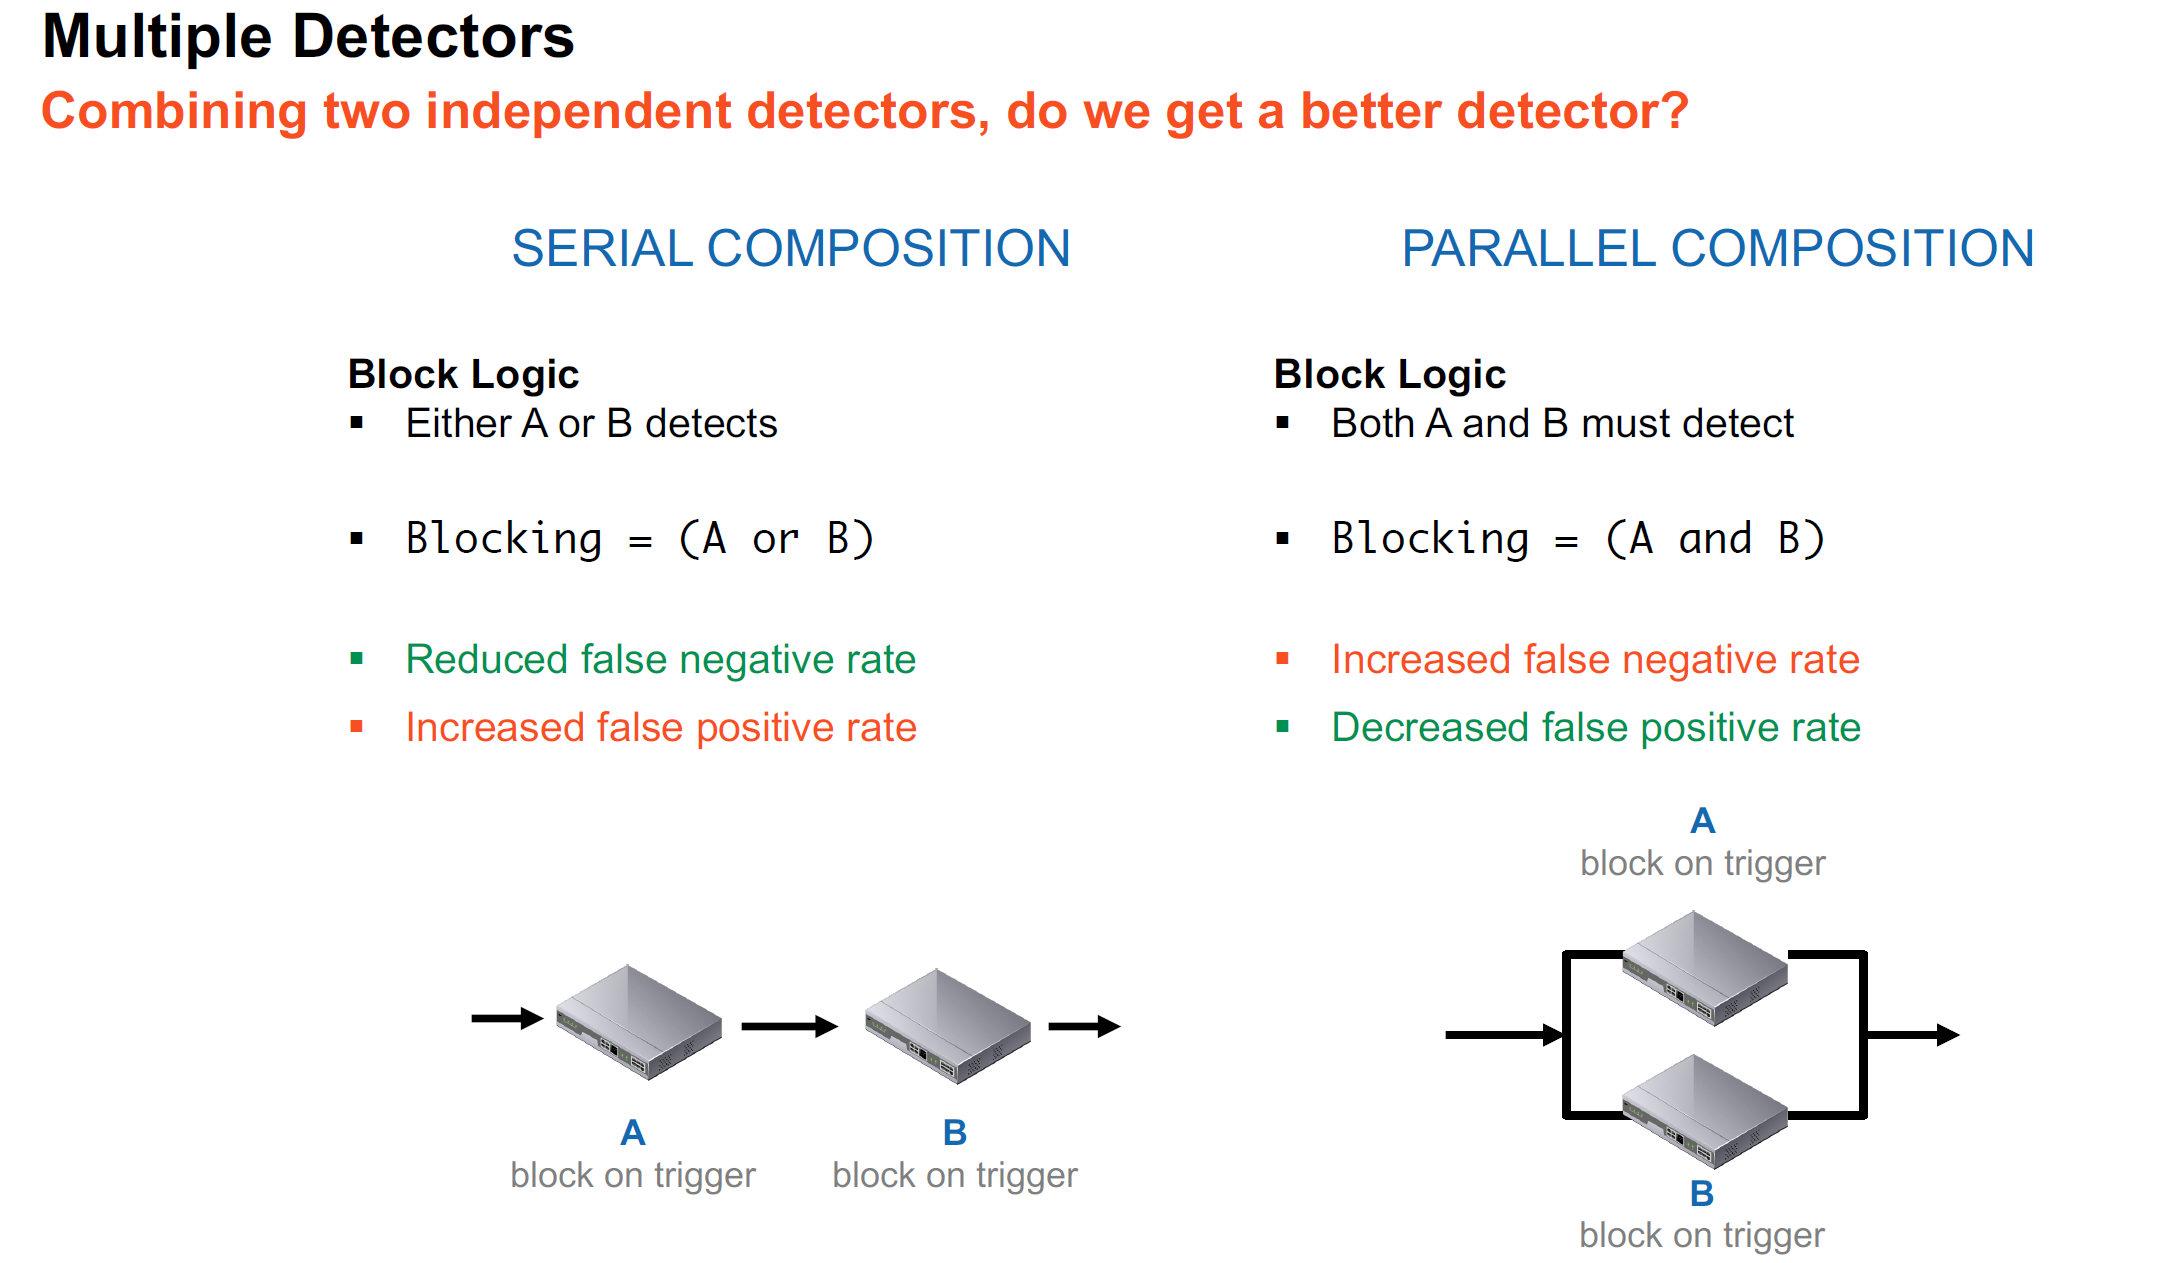
\includegraphics[width=\linewidth]{Figures/IDS_mult_detectors.PNG} 
\end{minipage}

\subsection{Layered Security Filtering and Protection:}

\begin{minipage}{\linewidth}
    \centering      
    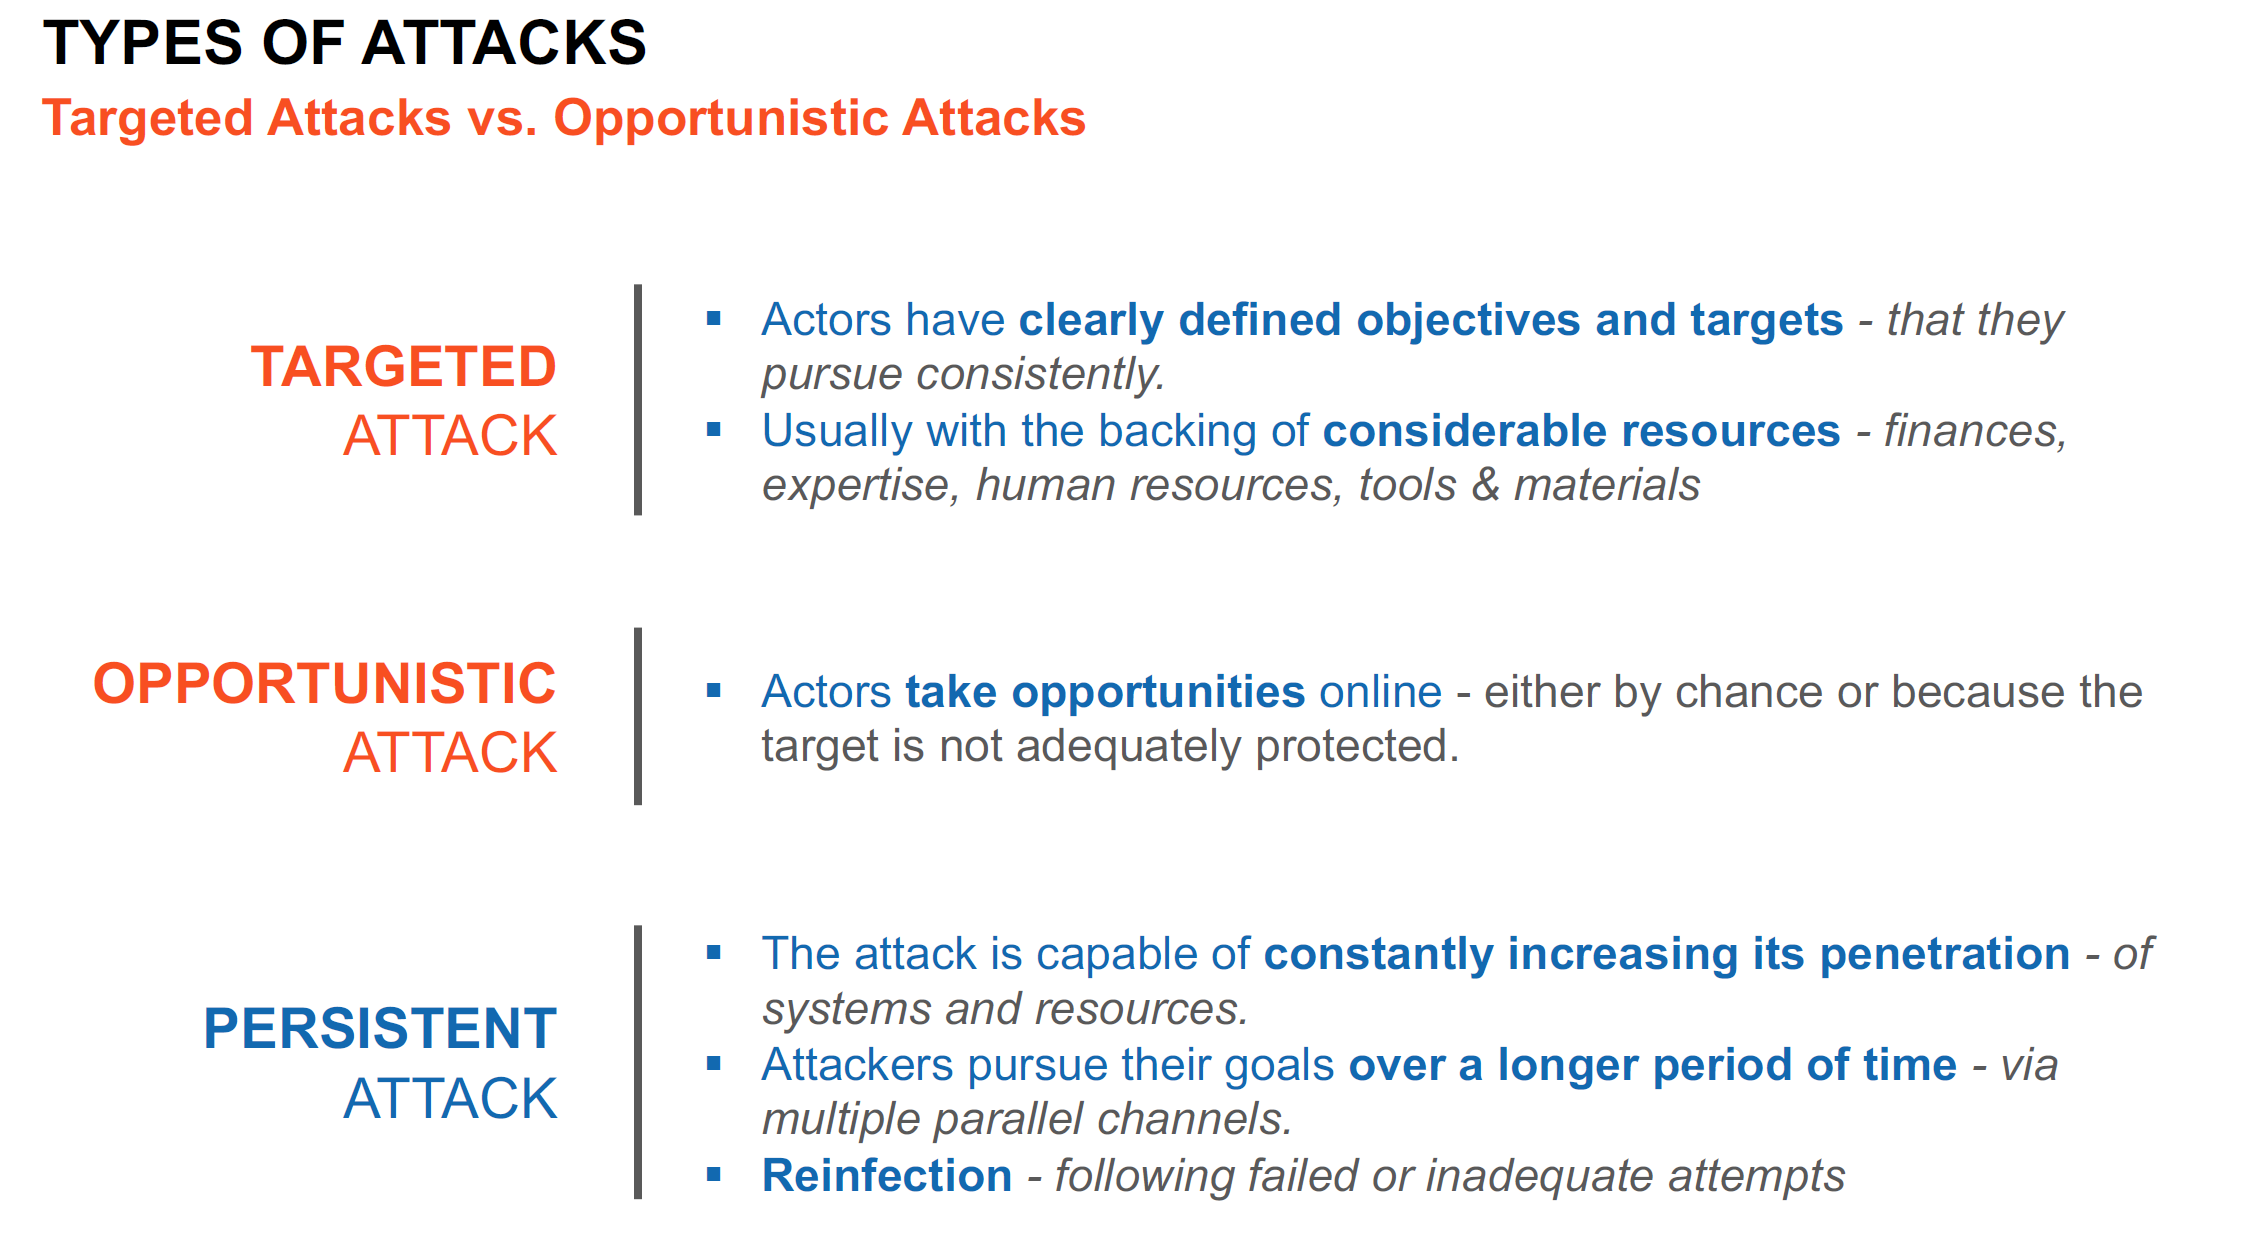
\includegraphics[width=\linewidth]{Figures/IDS_attack_types.PNG} 
\end{minipage}

\begin{minipage}{\linewidth}
    \centering      
    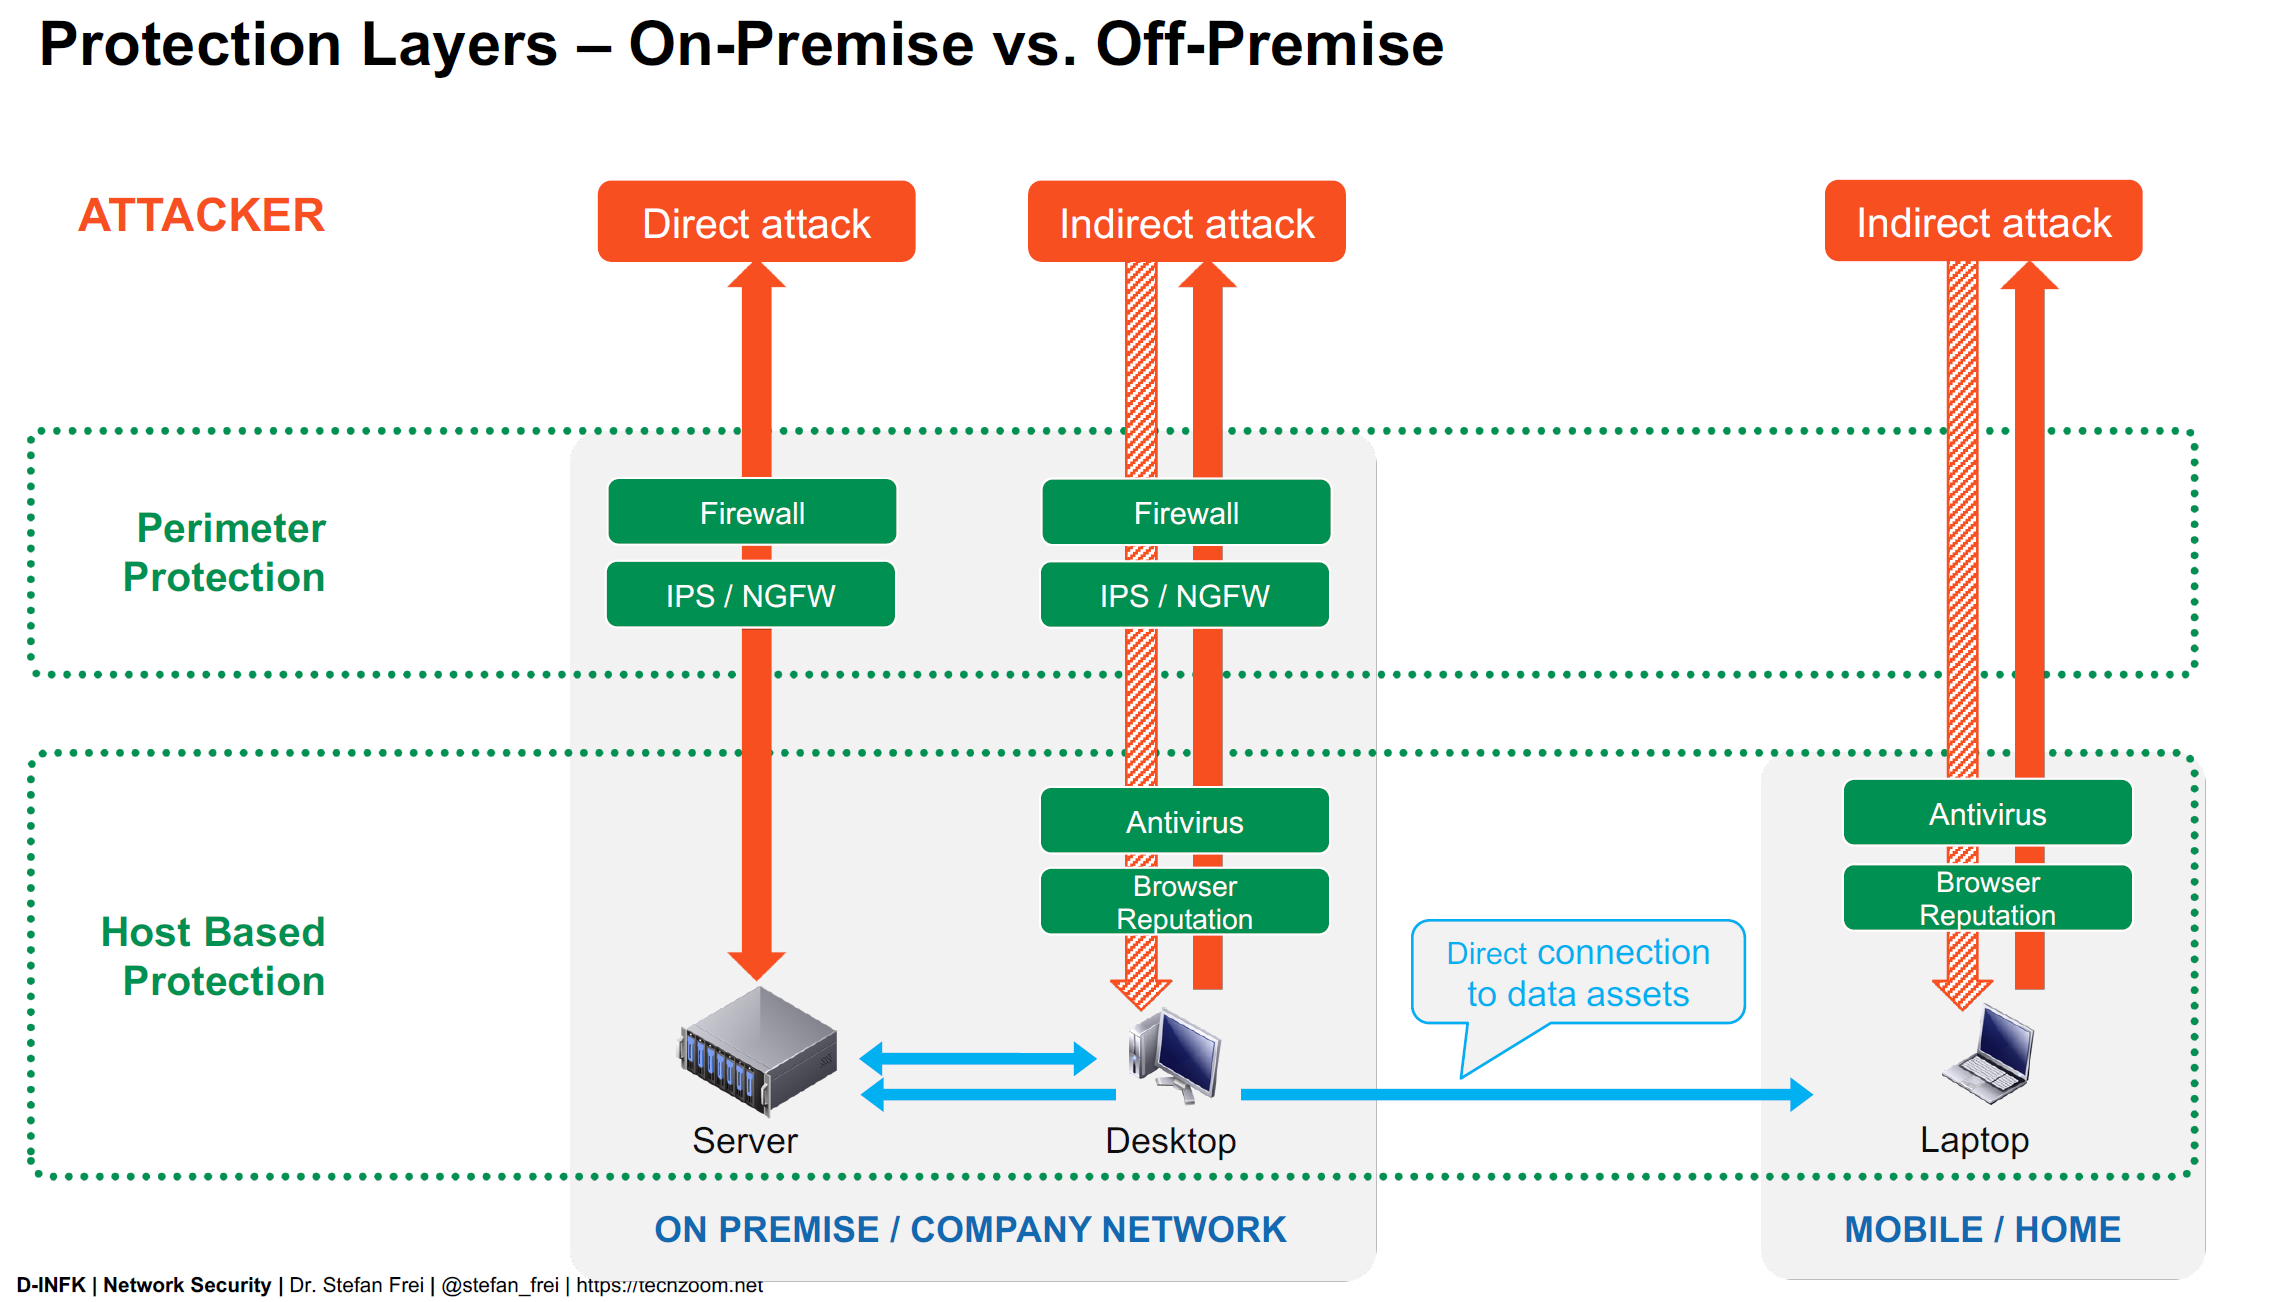
\includegraphics[width=\linewidth]{Figures/IDS_protection_layers.PNG} 
\end{minipage}

\begin{itemize}
	\item Direct attack: “server-side” exploits, the threat/exploit is executed remotely by the attacker against a vulnerable application and/or operating system
	\item Indirect attack: the threat/exploit is initiated by the vulnerable target. The attacker has little or no control over when the target user executes the threat.
\end{itemize}

\begin{minipage}{\linewidth}
    \centering      
    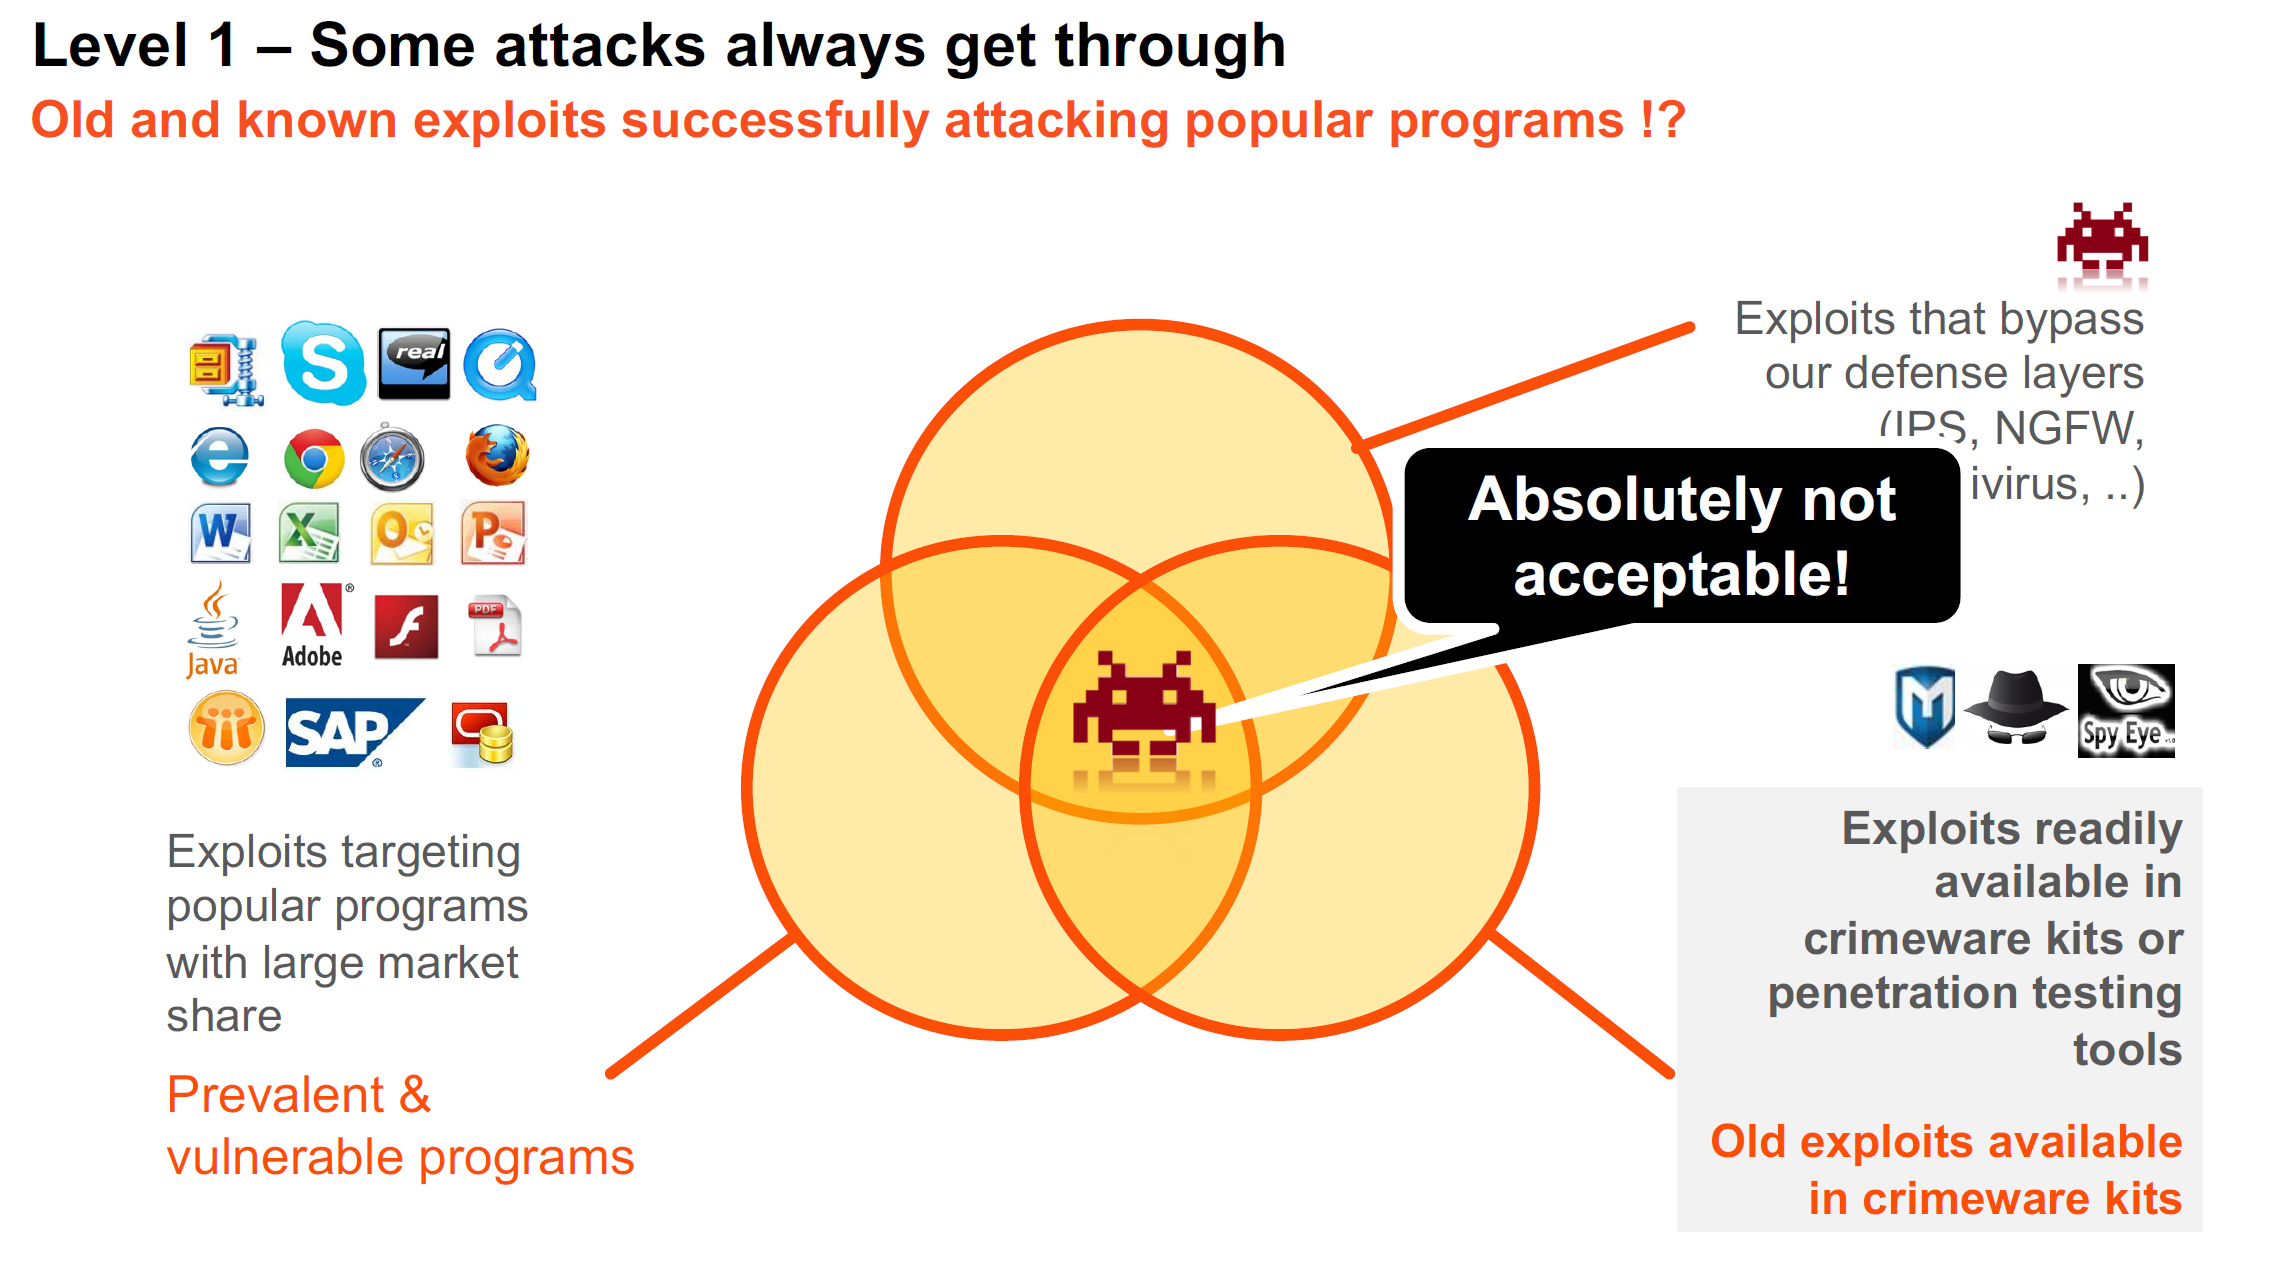
\includegraphics[width=\linewidth]{Figures/IDS_attack_model.PNG} 
\end{minipage}

\subsection{Botnets}

\paragraph{Basic components:}

\begin{itemize}
	\item Bots: devices under control of the attackers – often vulnerable hosts that have been
	infected with a malware.
	\item Command and Control infrastructure: often owned by the attackers, is it used to push
	commands to the bots.
\end{itemize}

\subsubsection{Mirai botnet}
\label{mirai_botnet}

Mirai mainly targeted IoT devices. IoT devices are a very interesting attack vector since there are lots of IoT devices (ca. 10 billion for 2019), they are configure-and-forget (owners don't update them and don't realize when they're compromised) and security is often lacking in IoT devices.\\
Mirai has been used mainly for Distributed Denial of Service attacks. DDoS is much harder to track and take down than a regular DoS. This allows the attacker to hide his identity behind the botnet. Additionally, a DDoS enables the attacker to have a virtually unlimited bandwidth for flood attacks.\\
Mirai infection technique:

\begin{enumerate}
	\item Scan: infected device scans network for open Telnet ports (send TCP SYN packets to random IPv4 addresses)
	\item Brute force: the bot tries to log in using 10 random user/pass combinations taken from
	a hardcoded list of 62. These represent default credentials of existing devices.
	\item Report: upon login success, the bot reports the target to a Report Server. It lists IP
	address, type of device (if available) and successful credentials.
	\item Infection: a Loader program gets a detail of the target from the Report Server, connects
	to Telnet and uploads the correct malware binary to the machine.
\end{enumerate}

Mirai is non-persistent: the binary is loaded into memory and immediately deleted from disk. Rebooting will remove the malware, but the device can still be reinfected. This makes detection and forensic analysis more difficult, especially for IoT devices.\\
Mirai infected devices were fingerprinted by the fact that Mirai generated probe packets had their sequence number equal to the IP of the scanned device. Probability of this happening is $\frac{1}{2^{32}}$.

\subsection{Stuxnet}

Stuxnet is the first (publicly know) cyberweapon - a complex malware, widely believed to have targeted uranium enrichment infrastructure in Iran. Stuxnet used various infection vectors such as WinCC machines, network shares, print spooler zero-day, removable drives (to jump airgaps). Stuxnet installed a driver, signed with a legitimate Realtek certificate. This driver intercepts I/O requests, making the files installed by the malware invisible. It also registers as a boot start service, acting as load point at reboots. This driver behaves very much like a legitimate Windows driver: this, and its legitimate Realtek signature, make it very hard to detect even for an experienced sysadmin. Stuxnet would survive manual inspection, OS updates and antivirus scans. This required legitimate certificates. Using fake certificates would have also been possible but surviving system updates would become harder. Hiding in plain sight is often a winning strategy. Stuxnet often injected itself into the privileged antivirus process to ease the infection. Depending on the antivirus, it alternatively ignored it and injected itself in a Windows system process. 
